\chapter{Tau Lifetime Studies}

\section{Motivation}

One of the most significant challenges faced in searches for heavy resonances decaying to tau pairs is the presence of neutrinos in the tau decays. Hadronic tau decays produce one neutrino, and leptonic tau decays produce two neutrinos so that, depending on the channel studied, each di-tau event may have two, three, or four neutrinos present in the decay products. These neutrinos do not interact with the detector, and carry energy away from the event. Information about the neutrinos can only be inferred from $\MET$, an event-level (as opposed to particle-level) quantity which estimates the net (event-wide) neutrino momentum in the transverse direction. If, for example, two neutrinos are produced back-to-back, the only recoverable information about them is the net difference in transverse momentum. Given that the taus, and by extension their decay products, are generated back-to-back (in the transverse plane) in $Z^\prime$ decays, $\MET$ alone does not provide sufficient information to precisely model the di-tau mass. The current mass estimator used in the 8 TeV and 13 TeV $Z^\prime\to\tau\tau$ searches, $\massvis$, depends on $\MET$ and, as shown in Figure \ref{fig:massVisSigVsMC}, suffers due to this loss of information.

\begin{figure}[tbh!]
\centering
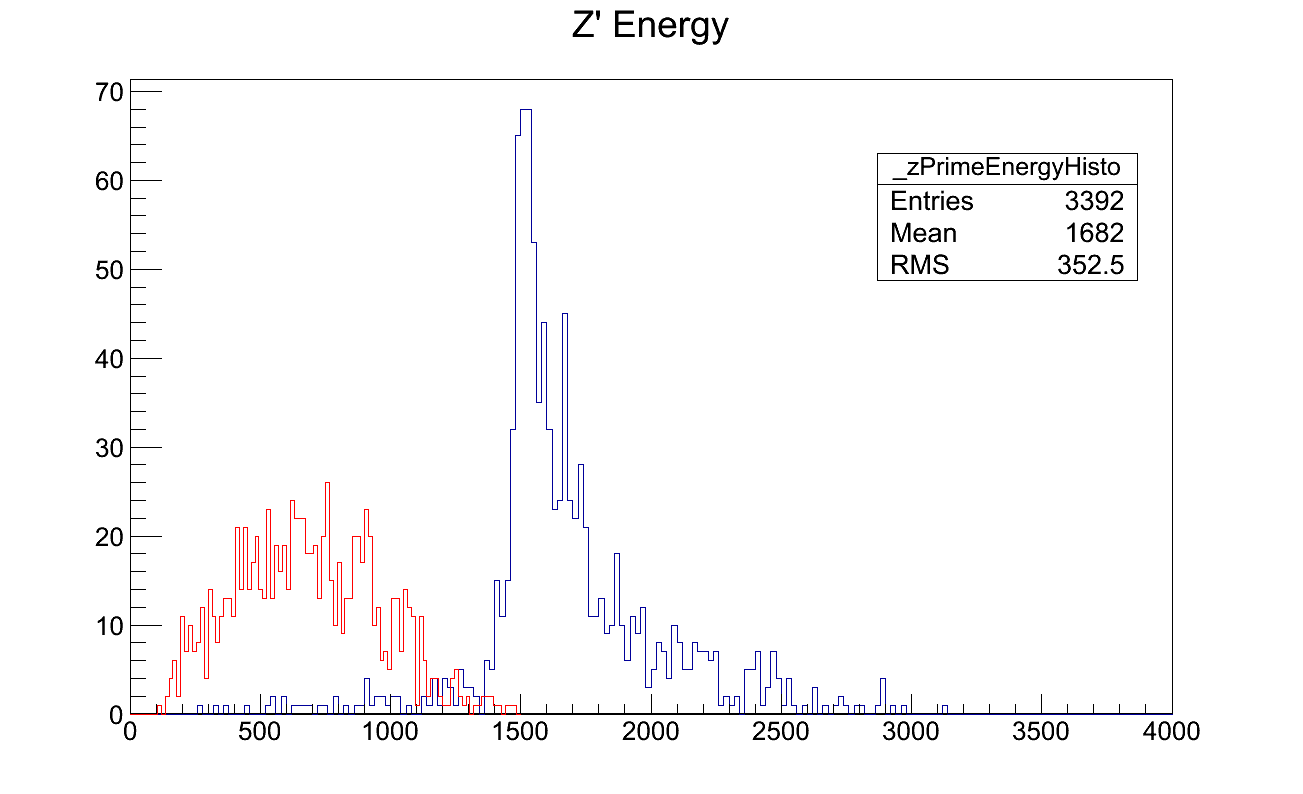
\includegraphics[width=0.6\textwidth]{figures/ZPrime1500EnergyMassVisOverlay.png}
\caption{1.5 TeV $Z^\prime$ generated energy (blue) compared to reconstructed visible mass, $\massvis$ (red). The $\massvis$ distribution is broader and peaked at a much lower energy than the MC truth.}
\label{fig:massVisSigVsMC}
\end{figure}

One proposal to improve the discriminating power of these searches is to add additional selection criteria taking advantage of the lifetime of the tau. At $2.9\times 10^{-13}$s, the tau lifetime is quite short, but it is still long enough to distinguish decay products originating from the primary vertex (PV) from those originating from the tau decay vertex. Essentially, ``prompt" particles coming directly from the PV leave tracks that may be traced back to the PV, while tracks from particles coming from tau decays will ``miss" the PV due to the distance the tau traveled from the PV before decaying. This concept is illustrated in Figure \ref{fig:PromptVsTauDecay}. These additional selection critera, referred to as ``lifetime cuts," are based on tracking information collected from the tau decay products.

\begin{figure}[tbh!]
\centering
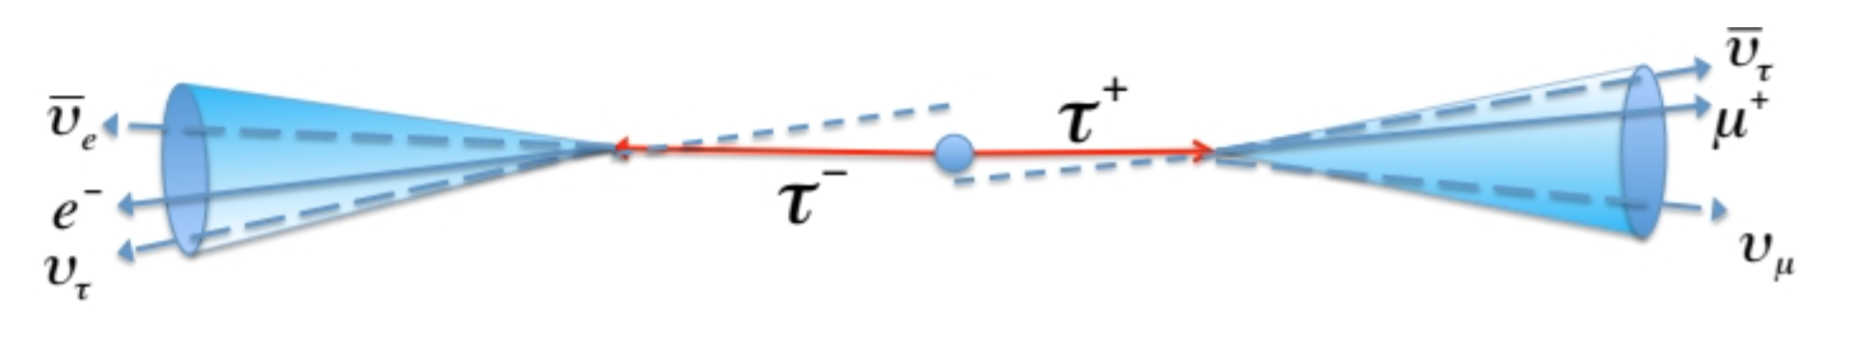
\includegraphics[width=1.0\textwidth]{figures/DiTauDecay.png}
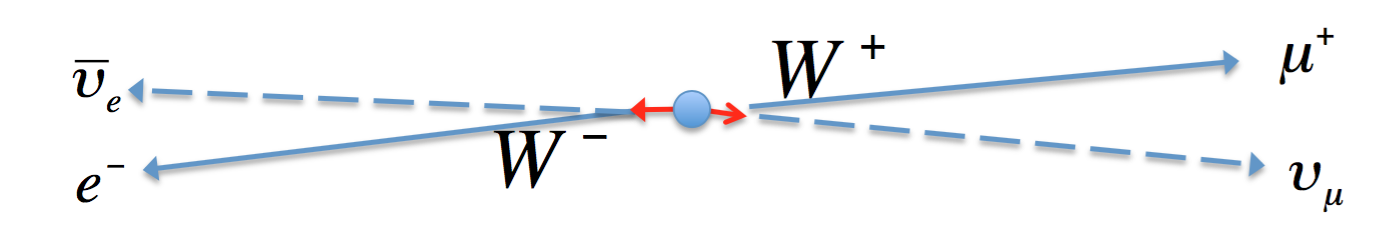
\includegraphics[width=1.0\textwidth]{figures/WWDecay.png}
\caption{A ditau event (top) will produce decay products whose tracks miss the PV, whereas leptonic decays from a shorter-lived parent produced in the $pp$ collision, such as a $W^+W^-$ event (bottom), will produce ``prompt" leptons which can be traced back to the PV.}
\label{fig:PromptVsTauDecay}
\end{figure}

\section{Methods}

Efforts to study the efficacy of the tau lifetime cuts began in the $\emu$ channel with a simple cut on the individual impact parameters (IPs) of the electron and muon in each ditau event. In this case, IP is defined as the closest distance between the track and a point with the x- and y-coordinates of the beam spot (BS) and the z-coordinate of the PV. The beam spot is a fixed quantity indicating the coordinates of the beam, and the PV is a quantity that is reconstructed from tracks in each event. In this channel, the principal prompt backgrounds are $t\bar{t}$, where the $b$ quarks from $t$ decays decay leptonically into an electron and muon, and $W^+W^-$, where the $W$s decay leptonically into an electron and muon. Drell-Yan events where virtual $Z$ bosons decay into tau pairs are in principle an irreducible background, but the rate falls off significantly in the high-mass (signal) region being considered.

The cut was first defined as the sum of the absolute values of the IPs of each lepton:

\begin{equation}
\centering
\textrm{Lifetime}_\tau = |\textrm{IP}_e| + |\textrm{IP}_\mu|
\end{equation}

\noindent To account for the large variance in track resolution, and thus prefentially-select ``clean" tau decays, the lifetime definition was modified to include the track measurement error:

\begin{equation}
\centering
\textrm{Lifetime}_\tau = \sqrt{\frac{\left(|\textrm{IP}_e| + |\textrm{IP}_\mu|\right)^2}{\sigma_{\textrm{IP}_e}^2 + \sigma_{\textrm{IP}_\mu}^2}}
\label{eq:IP}
\end{equation}

\noindent where the error on the track IP is defined according to the recommendations laid down by the Tracker POG\cite{TrackerPOG}:

\begin{equation}
\centering
\sigma_e = \textrm{abs(theGSFElec.gsfTrack()-$>$dxy(theBeamSpot))}
\end{equation}
\begin{equation}
\centering
\sigma_\mu = \textrm{abs(thePatMuon.track()-$>$dxy(theBeamSpot))}
\end{equation}

The cut is placed at the very end of the selection sequence, immediately following the b-jet veto. The quantity in Equation \ref{eq:IP} is required to exceed a value chosen based on optimization studies. These studies, based in signal and background MC, compare the acceptance of signal events with the rejection of background events across several values of this threshold. The threshold value is chosen based on its associated value of $\frac{s}{\sqrt{s+b}}$, where $s$ is the signal rate and $b$ is the aggregated background rate. Figure \ref{fig:IPstudy} shows the performance of the IP-based lifetime cut in MC. A cut threshold of 2 is chosen on the basis of maximizing both $\frac{s}{\sqrt{s+b}}$ and signal MC acceptance.


\begin{figure}[tbh!]
\centering
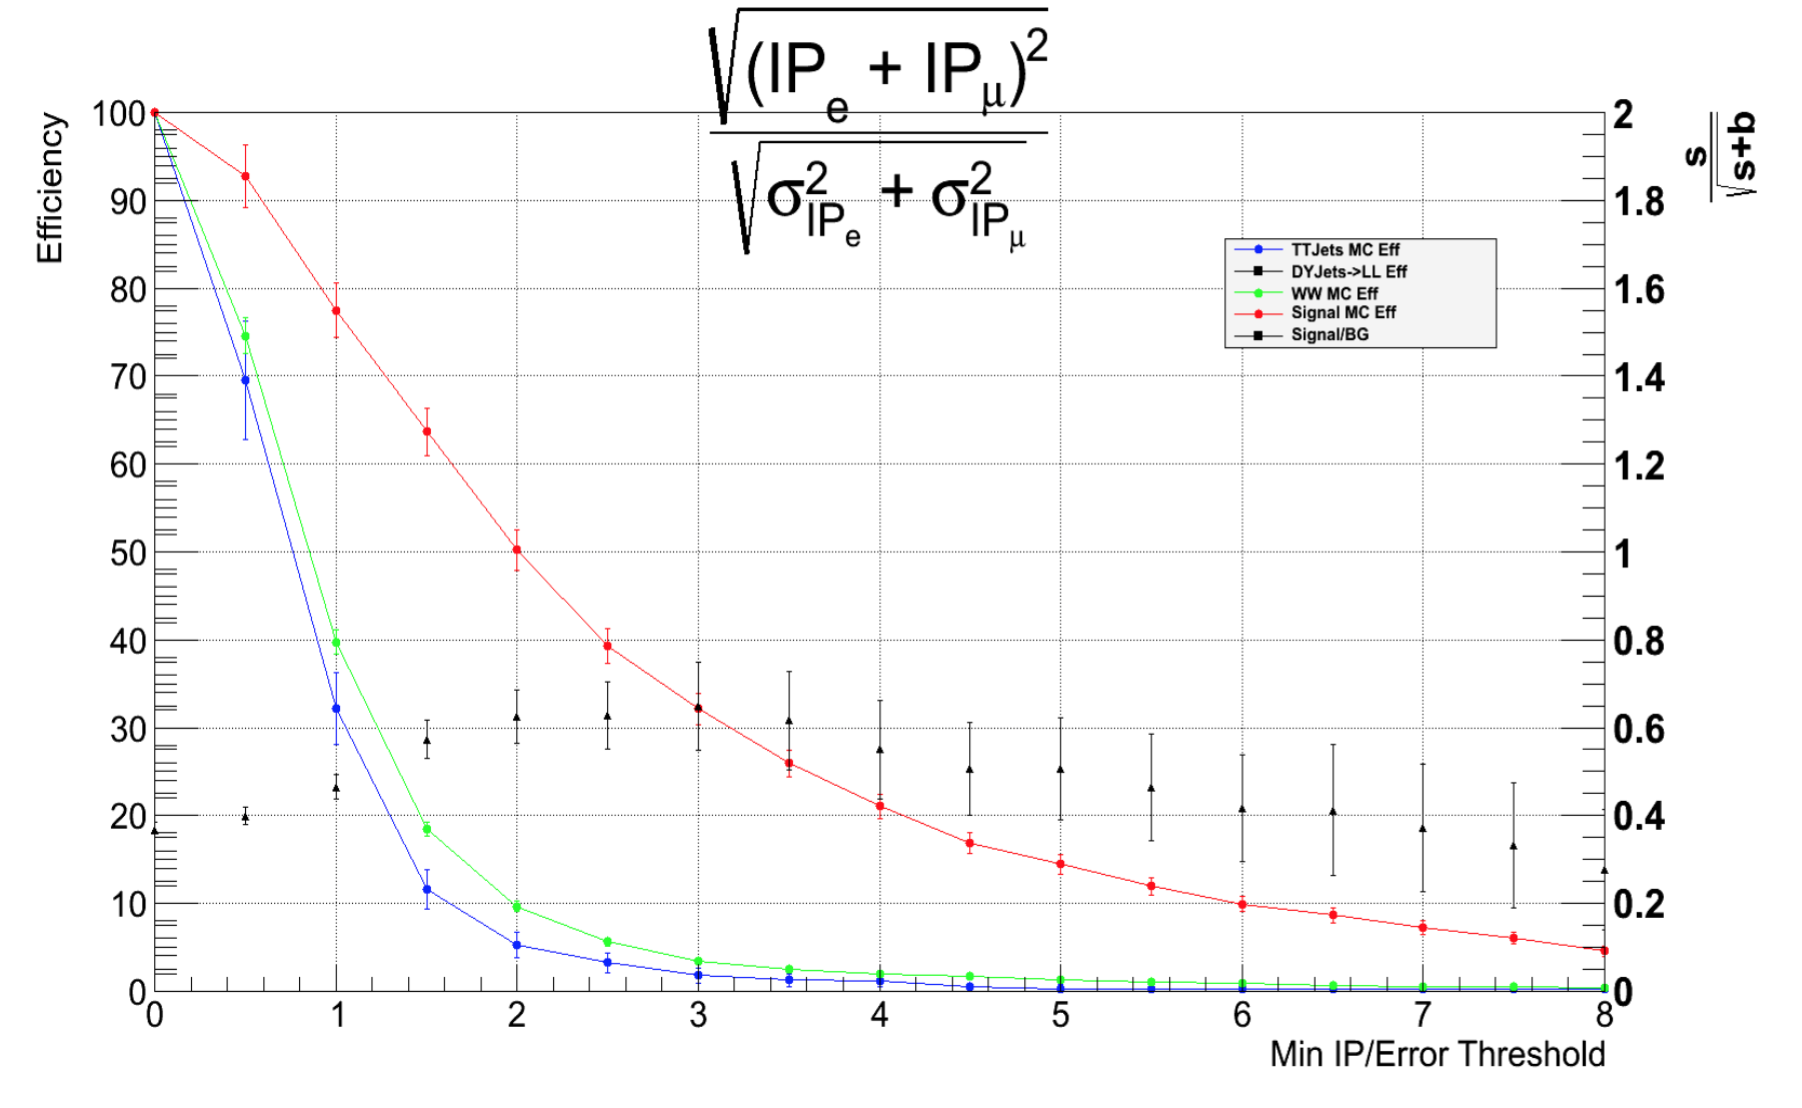
\includegraphics[width=1.0\textwidth]{figures/IPstudy.png}
\caption{Plot showing the performance of the IP definition of the lifetime cut. The colored lines indicate MC efficiencies and correspond to the left axis. The black triangles indicate $\frac{s}{\sqrt{s+b}}$ and correspond to the right axis. A threshold value of 2 was chosen for the cut since it is the first value on the plateau of $\frac{s}{\sqrt{s+b}}$ maxima, thereby keeping signal MC acceptance as high as possible.}
\label{fig:IPstudy}
\end{figure}


Another cut exploiting tau lifetime is one based on the distance-of-closest approach (DCA) between the two lepton tracks. DCA is defined to be the transverse distance between the two tracks at their point of closest approach. DCA is also divided by its error, where error on DCA is again defined according to the Tracker POG recommendation\cite{TrackerPOG}:

\begin{equation}
\centering
\sigma_{DCA} = \sqrt{\frac{\vec{DCA^T}\times M_\sigma\times\vec{DCA}}{|\vec{DCA}|^2}}
\end{equation}

\noindent where $M_\sigma$ is a 3x3 covariance matrix containing the x, y, and z-errors summed over the electron and muon points of closest approach. Figure \ref{fig:DCAstudy} shows the performance of the DCA/$\sigma$ cut.

\begin{figure}[tbh!]
\centering
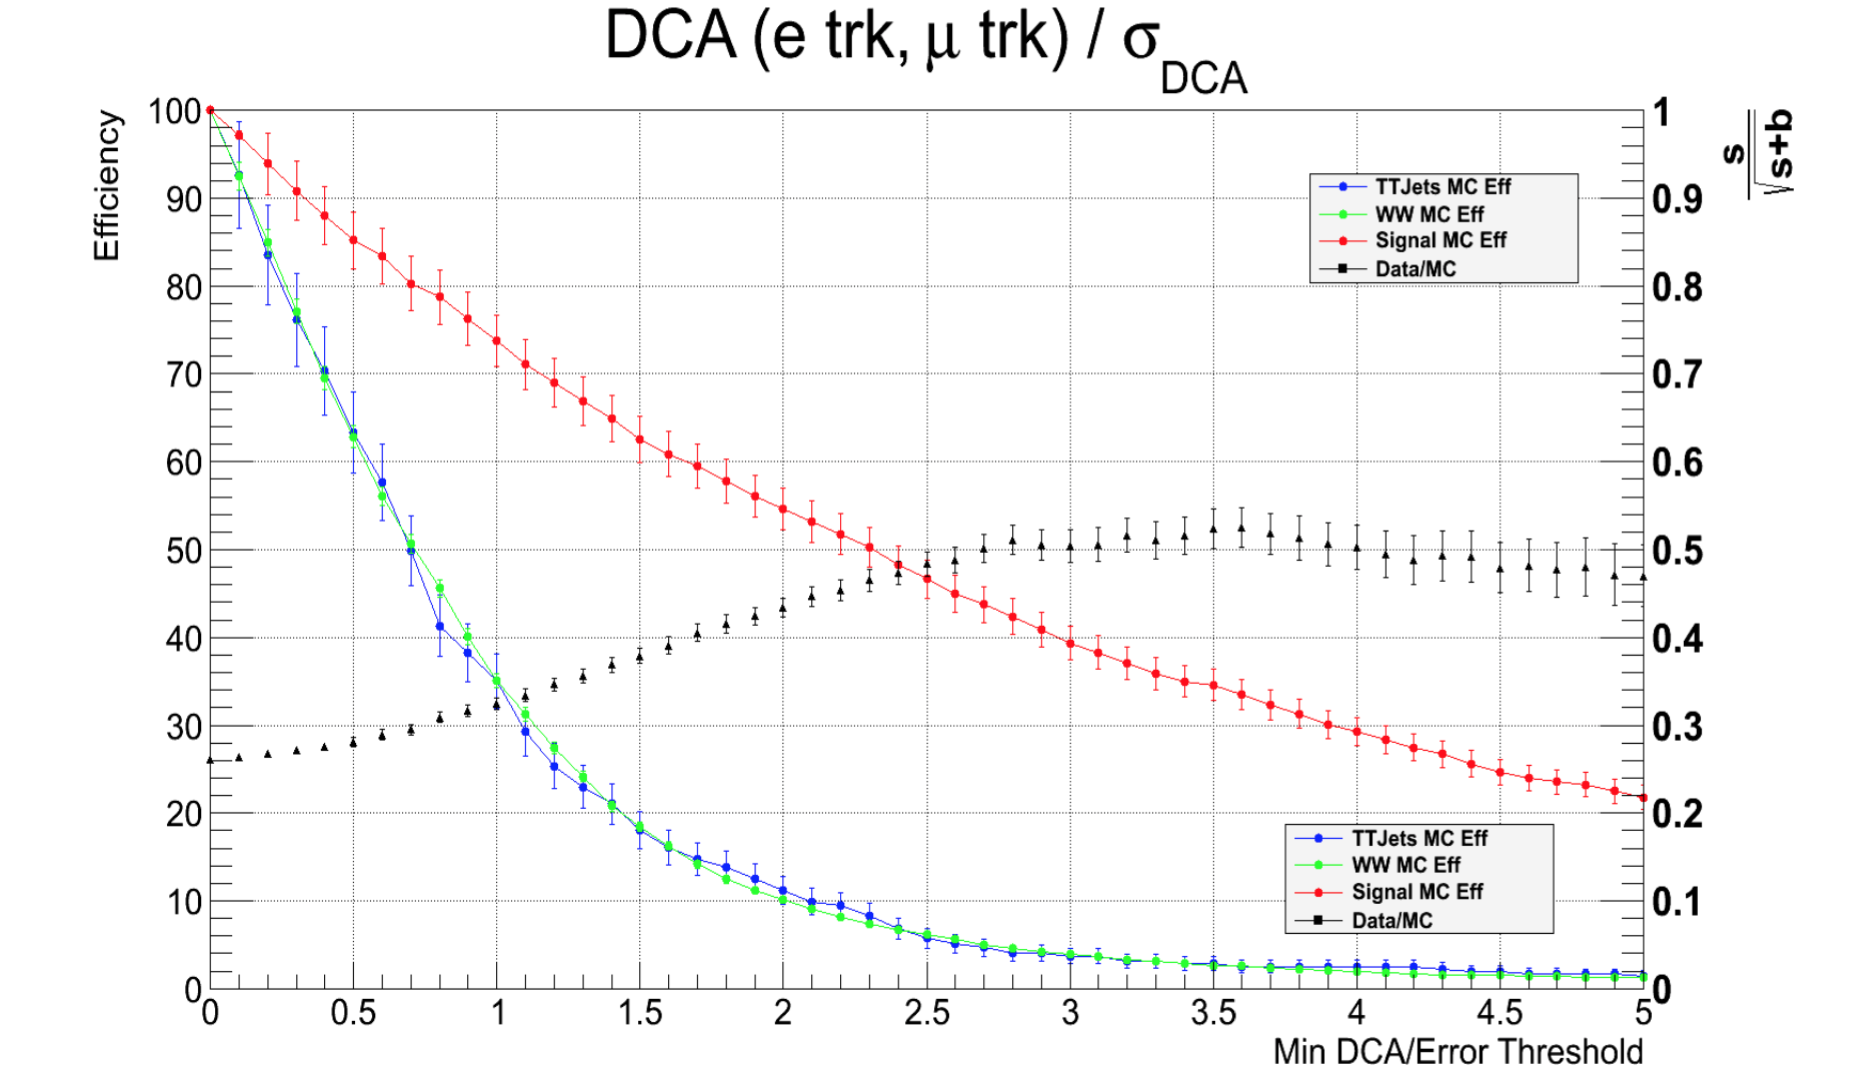
\includegraphics[width=1.0\textwidth]{figures/DCAstudy.png}
\caption{Plot showing the performance of the DCA definition of the lifetime cut. The colored lines indicate MC efficiencies and correspond to the left axis. The black triangles indicate $\frac{s}{\sqrt{s+b}}$ and correspond to the right axis. A threshold value of 2.5 was chosen for the cut since it is the first value on the plateau of $\frac{s}{\sqrt{s+b}}$ maxima, thereby keeping signal MC acceptance as high as possible.}
\label{fig:DCAstudy}
\end{figure}

The DCA cut has the potential to veto valid signal events in cases where the two lepton tracks are far from the BS/PV but close to one another (illustrated in Figure \ref{fig:DCAfail}). In such cases, the IP-based cut would still retain the signal event. Therefore, the final definition of the lifetime cut is the requirement that events pass the IP-based cut \emph{OR} the DCA cut. The performance of this ``OR" cut is shown in Figure \ref{fig:DCAorIPstudy}.

\begin{figure}[tbh!]
\centering
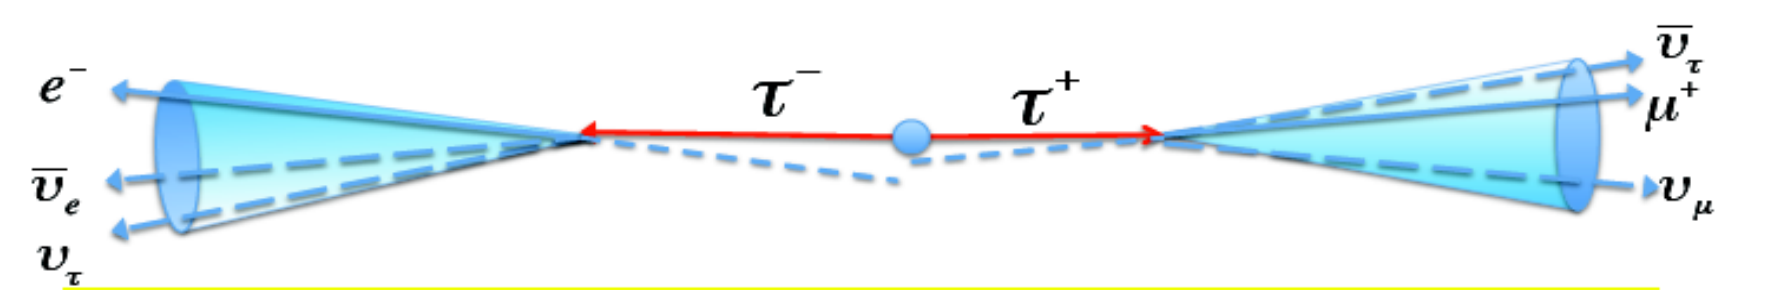
\includegraphics[width=1.0\textwidth]{figures/DCAfail.png}
\caption{Example of where the DCA cut could reject a valid signal event - the two lepton tracks have a low DCA despite a high IP}
\label{fig:DCAfail}
\end{figure}

\begin{figure}[tbh!]
\centering
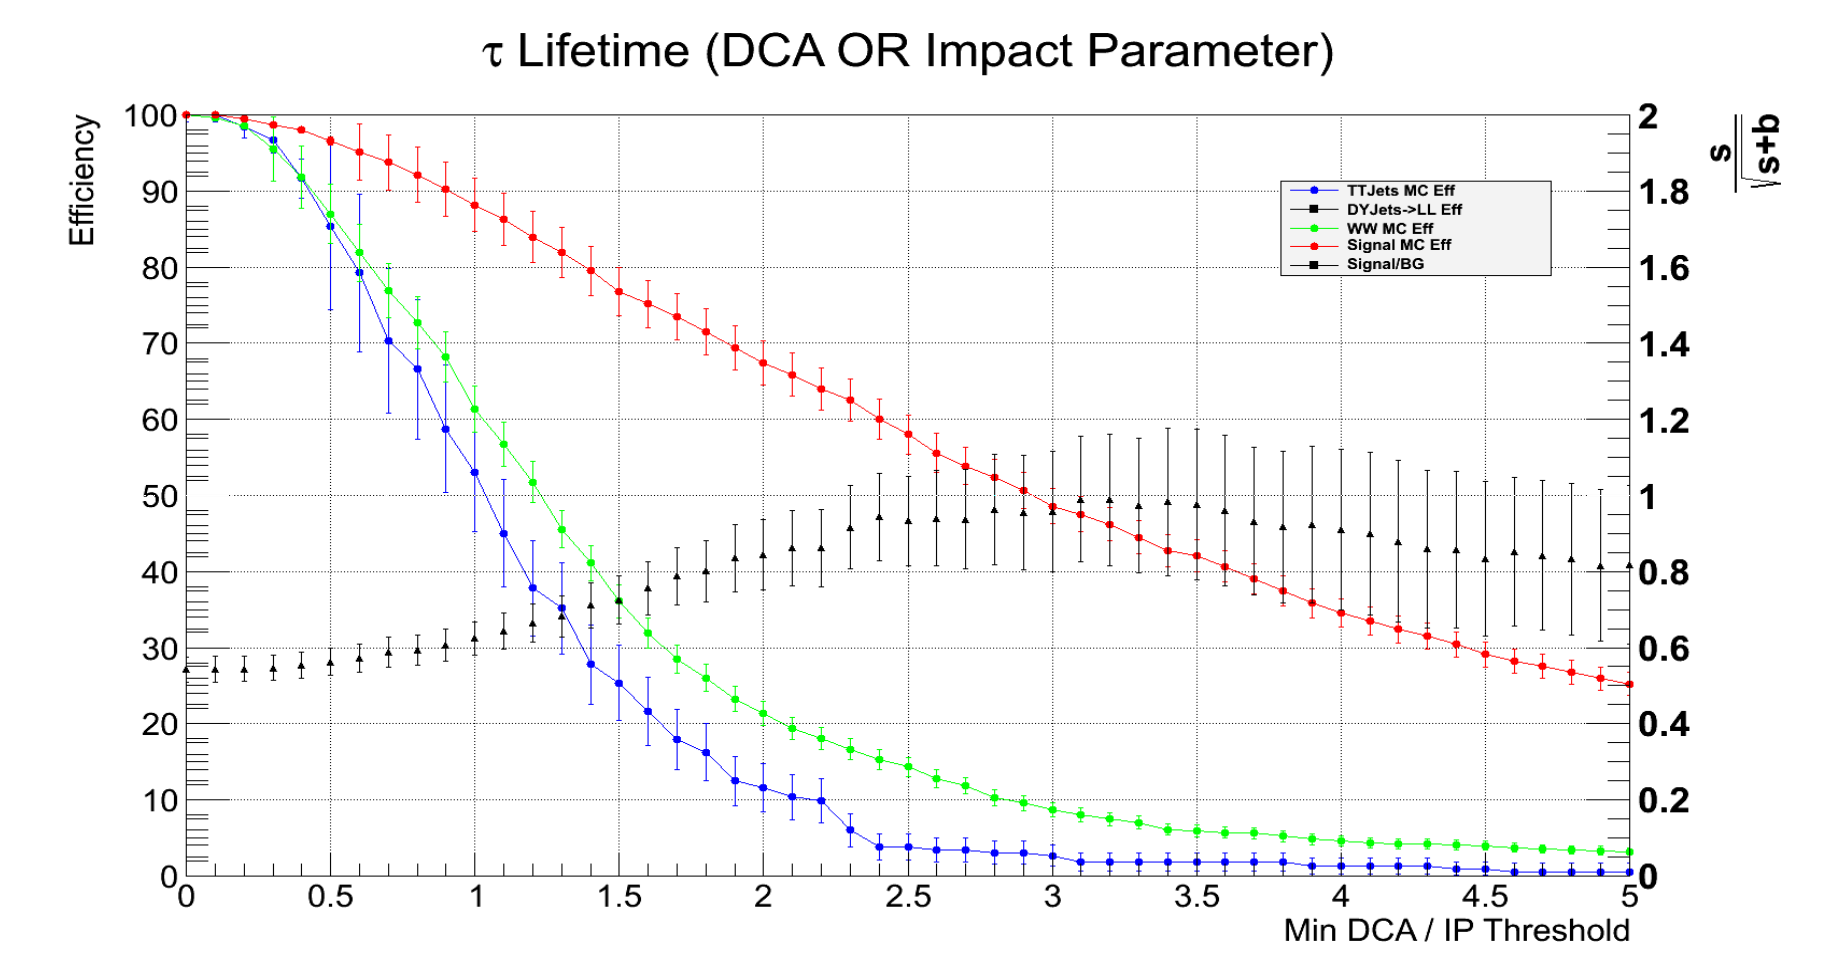
\includegraphics[width=1.0\textwidth]{figures/DCAorIPstudy.png}
\caption{Plot showing the performance of the DCA \emph{OR} IP-based definition of the lifetime cut. The colored lines indicate MC efficiencies and correspond to the left axis. The black triangles indicate $\frac{s}{\sqrt{s+b}}$ and correspond to the right axis. A threshold value of 2 was chosen for the cut since it is the first value on the plateau of $\frac{s}{\sqrt{s+b}}$ maxima, thereby keeping signal MC acceptance as high as possible. Note that the performance in this cut, in terms of signal acceptance and background rejection, is higher than either the IP-based or DCA cuts individually.}
\label{fig:DCAorIPstudy}
\end{figure}

\section{Impact on Limit}

\subsection{8 TeV Results in the $\emu$ Channel}

Figure \ref{fig:8TeVLifetimeLimits} shows the impact of the addition of the lifetime cut (``OR" definition) on the overall limit. Note that the limit without the lifetime cut shown in Figure \ref{fig:8TeVLifetimeLimits} is different from the final limit published in EXO-12-046 and shown in Section \ref{sec:results}. This is due to the fact that the lifetime study was performed early in the 8 TeV analysis when a different technique was being used for limit-setting. Namely, the limits shown here were produced with the Asymptotic $\textrm{CL}_{\textrm{s}}$ method\cite{HiggsCombine} using one datacard per background as input, while the final limits shown in EXO-12-046 used the full $\textrm{CL}_{\textrm{s}}$ method\cite{HiggsCombine} using one datacard per bin for each background. Despite the difference, it is still apparent that the addition of the addition of the lifetime cut improves the limit by $\sim70$ GeV.

\begin{figure}[tbh!]
\centering
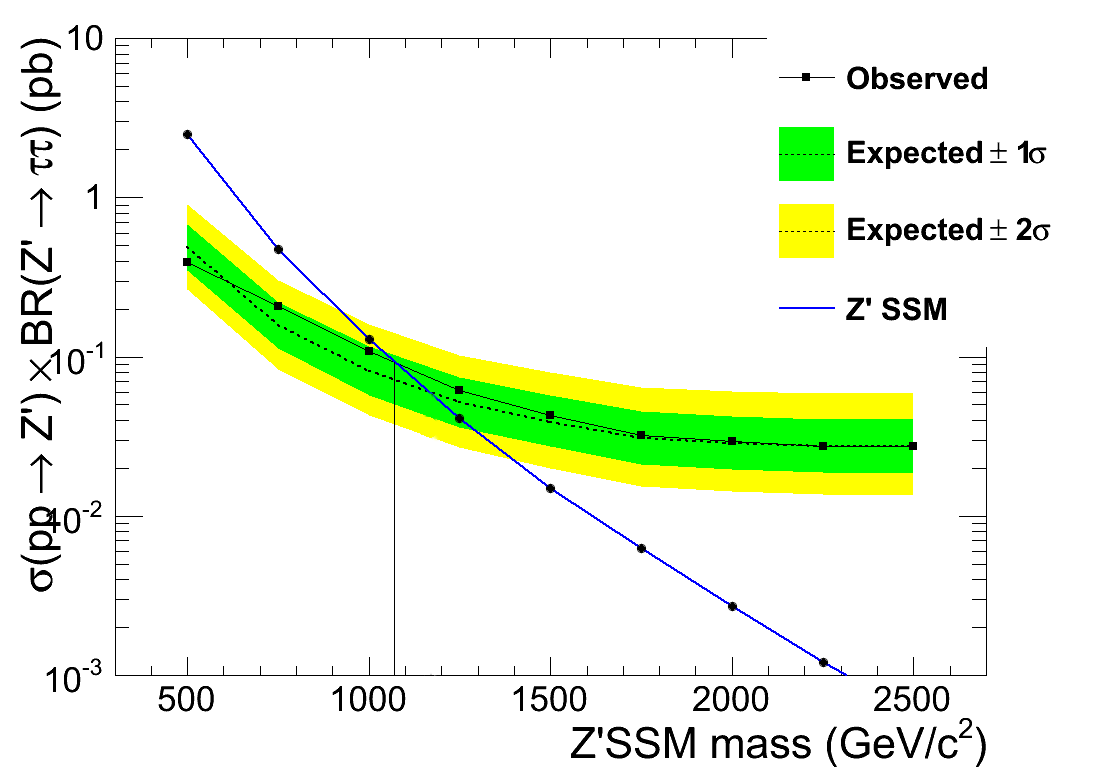
\includegraphics[width=0.5\textwidth]{figures/Limit_noLifetime_oneBG_6_5_14.png}
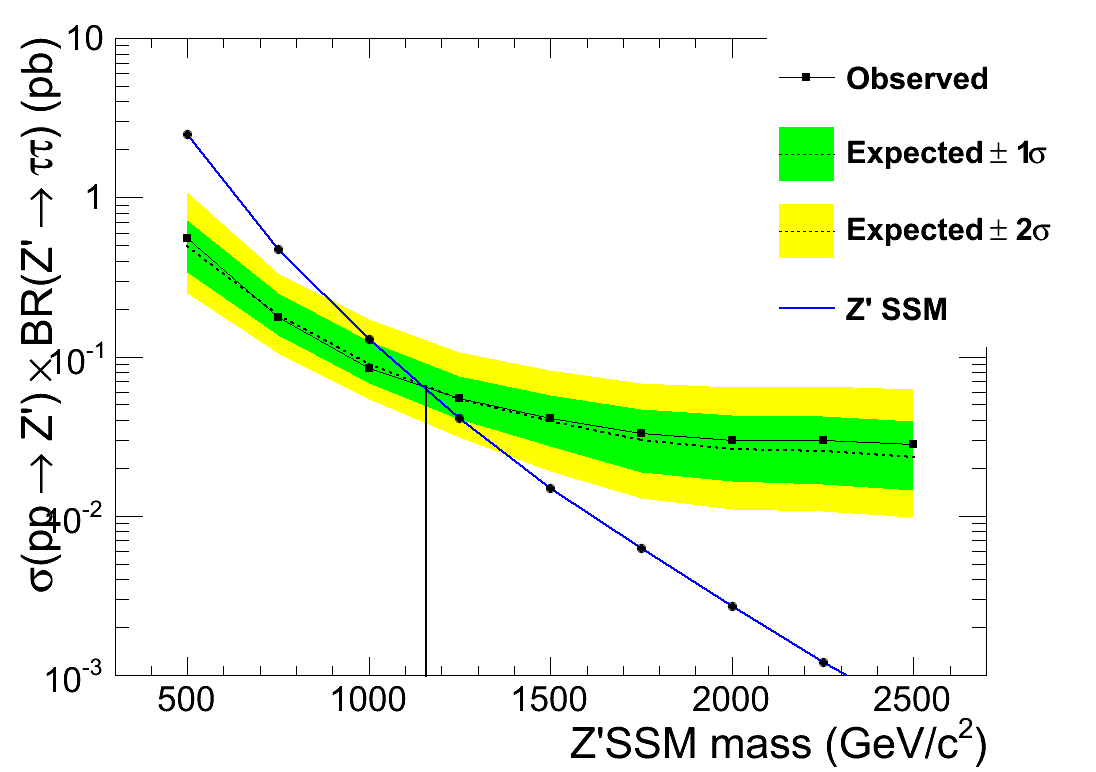
\includegraphics[width=0.5\textwidth]{figures/Limit_Lifetime_gt_2_oneBG_6_11_14.png}
\caption{Limit calculated with standard 8 TeV selection sequence (top) compared with limit calculated with the standard selection sequence and a lifetime threshold of 2 applied (bottom). The addition of the lifetime cut improves the exclusion limit by about 70 GeV.}
\label{fig:8TeVLifetimeLimits}
\end{figure}

\subsection{13 TeV Results in the $\thth$ Channel}

For the 13 TeV analysis, the focus of the lifetime study is shifted to the fully-hadronic $\thth$ channel, where the leading charged pion tracks from the hadronic tau decays are used in place of the electron and muon tracks. QCD is the overwhemingly dominant background in this channel (see Section \ref{sec:dihad}). Since QCD MC is not available, a full optimization study to determine the appropriate lifetime cut value is more difficult. Instead of a plot like Figure \ref{fig:DCAorIPstudy}, the distributions of combined IP/$\sigma$ are compared for a 2.5 TeV $Z^\prime\to\tau_h\tau_h$ sample in the signal region and for data in the same-sign QCD control region. In this case, data in the SS QCD CR is used as an approximation for QCD, given the relative dominance of QCD in this channel. Figure \ref{fig:13TeVComparison} shows this comparison, and a lifetime cut threshold of 3 is selected for this analysis.

\begin{figure}[tbh!]
\centering
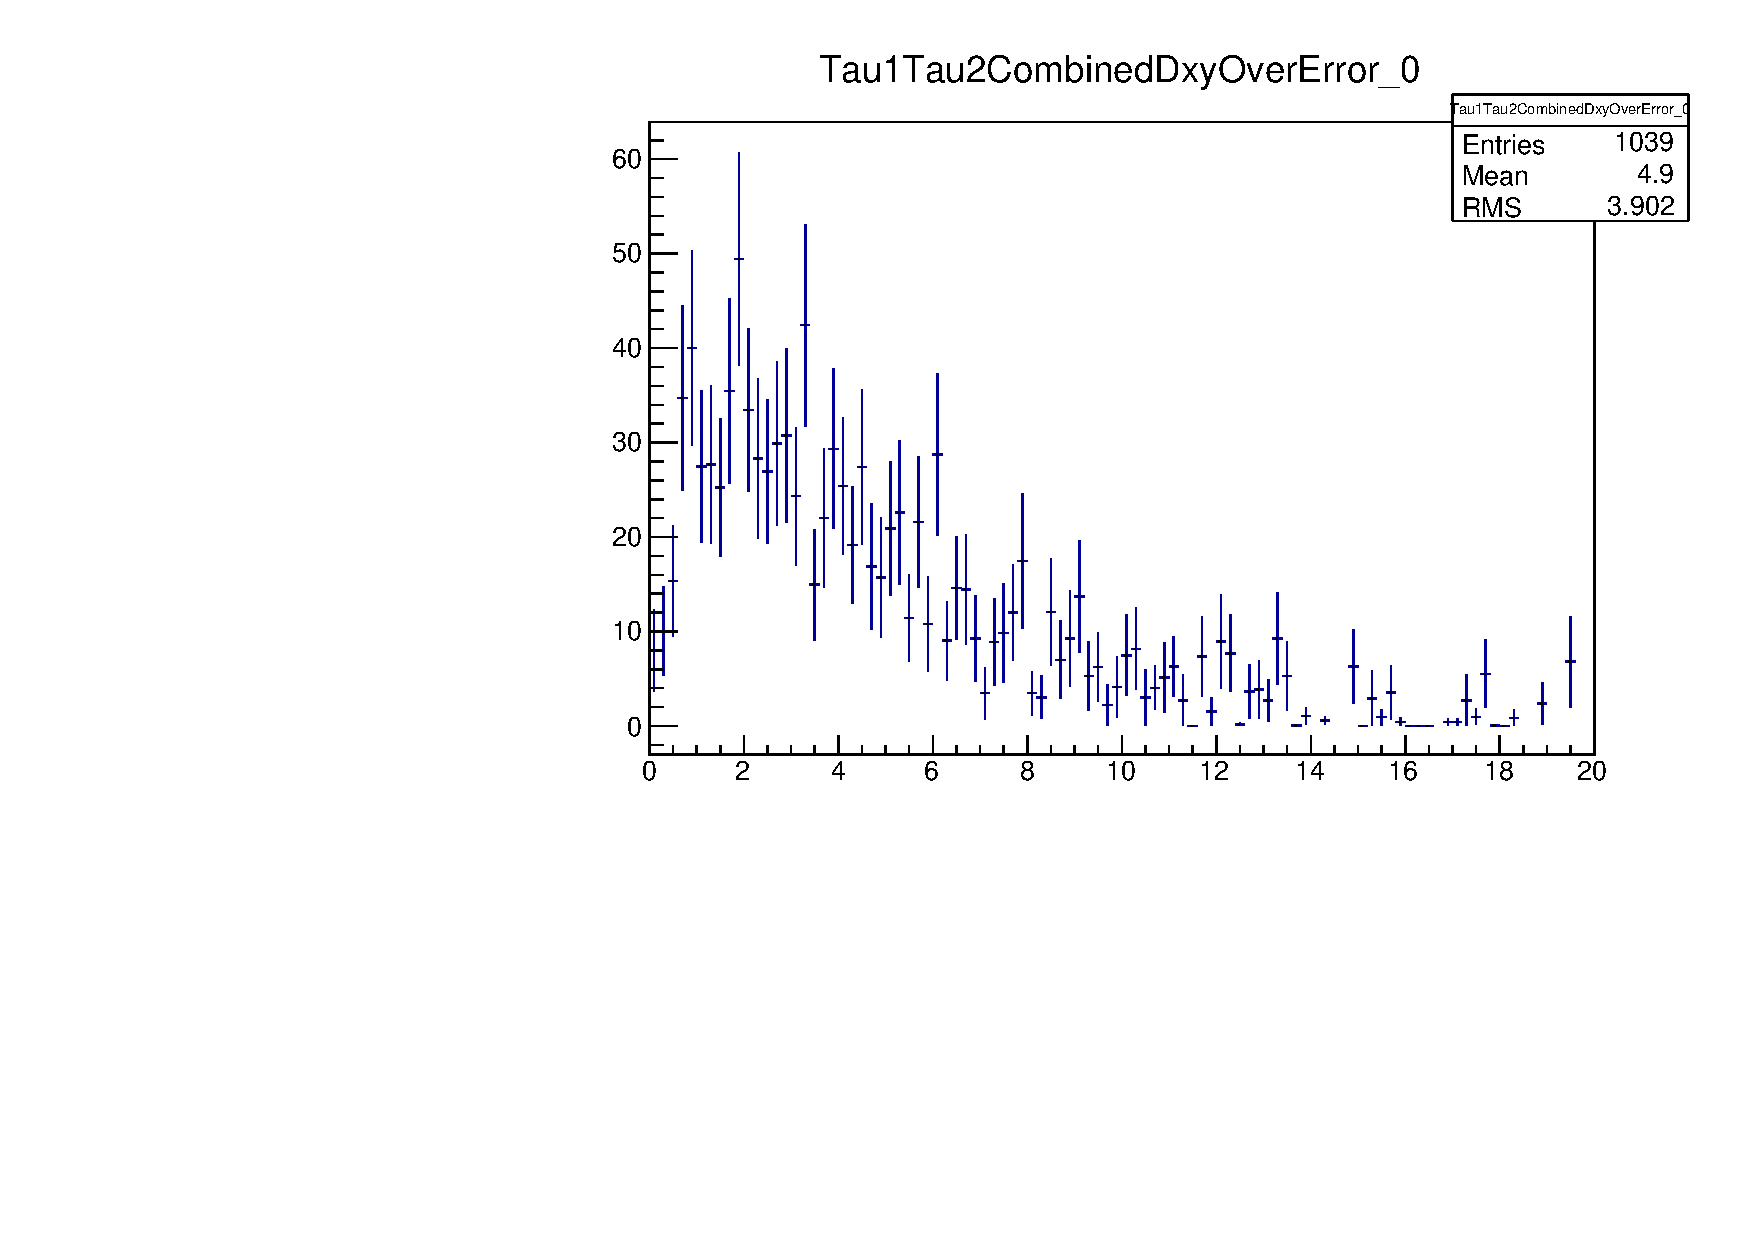
\includegraphics[width=0.5\textwidth]{figures/Zprime_2500GeV_CombinedDxyOverError.pdf}
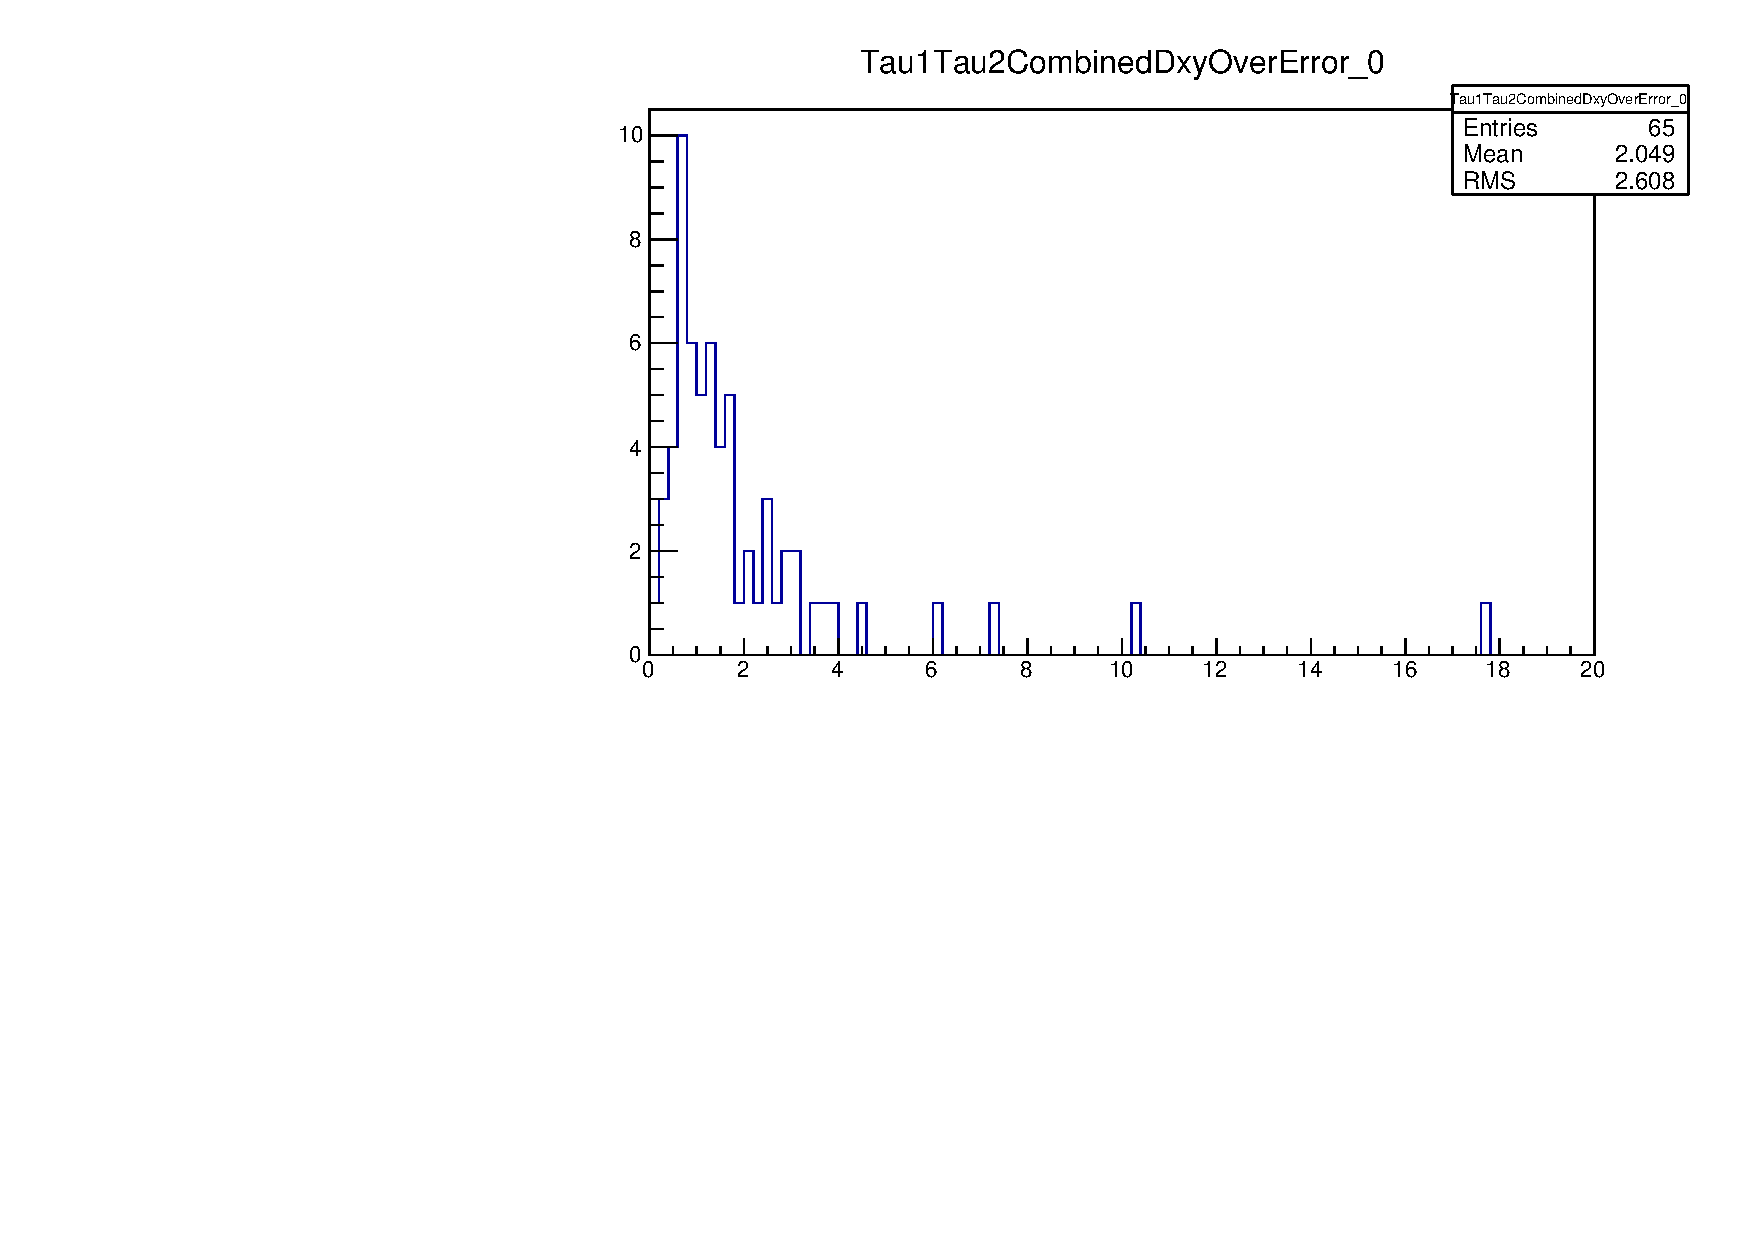
\includegraphics[width=0.5\textwidth]{figures/Data_CombinedDxyOverError.pdf}
\caption{Distribution of combined IP/$\sigma$ for a 2.5 TeV $Z^\prime\to\tau_h\tau_h$ sample in the SR (top) and data (used as a proxy for QCD) in the SS QCD CR (bottom). A threshold value of 3 is selected for the limit comparison.}
\label{fig:13TeVComparison}
\end{figure}

Figure \ref{fig:13TeVLifetimeLimits} shows the impact of the addition of the lifetime cut (``OR" definition) on the overall limit. In this channel and at this collision center-of-mass energy, the addition of the lifetime cut appears to decrease both the expected and observed limits by $\sim$100 GeV. It's likely that the extremely low event rates in the high mass region (i.e. the search region with the highest sensitivity) is what drives this behavior. Since the background rate in the high mass region is already quite low, the fact that the lifetime cut rejects $\sim$50\% of the signal is likely to have a larger impact on the limit than boosting the signal-to-background ratio. In an effort to increase signal events in this region, the $p_\zeta$ cut was removed. However, this alone permitted a significant increase in QCD background, so the $\MET$ cut was tightened to $\MET > 50$. The results are shown in Figure \ref{fig:13TeVImprovedLimits}. These modifications appear to increase the baseline limit. However, even with increased statistics, the addition of the lifetime cut appears to decrease the limit relative to the limit without the lifetime cut. The conclusion is that, in the high-mass region, the loss of signal events due to the lifetime cut affects the limit sensitivity more than the concurrent suppression of background. The lifetime cuts will once again be tested as statistics accumulate during the 2016 run and beyond. Multivariate analysis (MVA) techniques will also be applied so that these new cuts can be fully integrated and properly ``tuned" with the rest of the $Z^\prime\to\tau\tau$ selection cuts.

\begin{figure}[tbh!]
\centering
%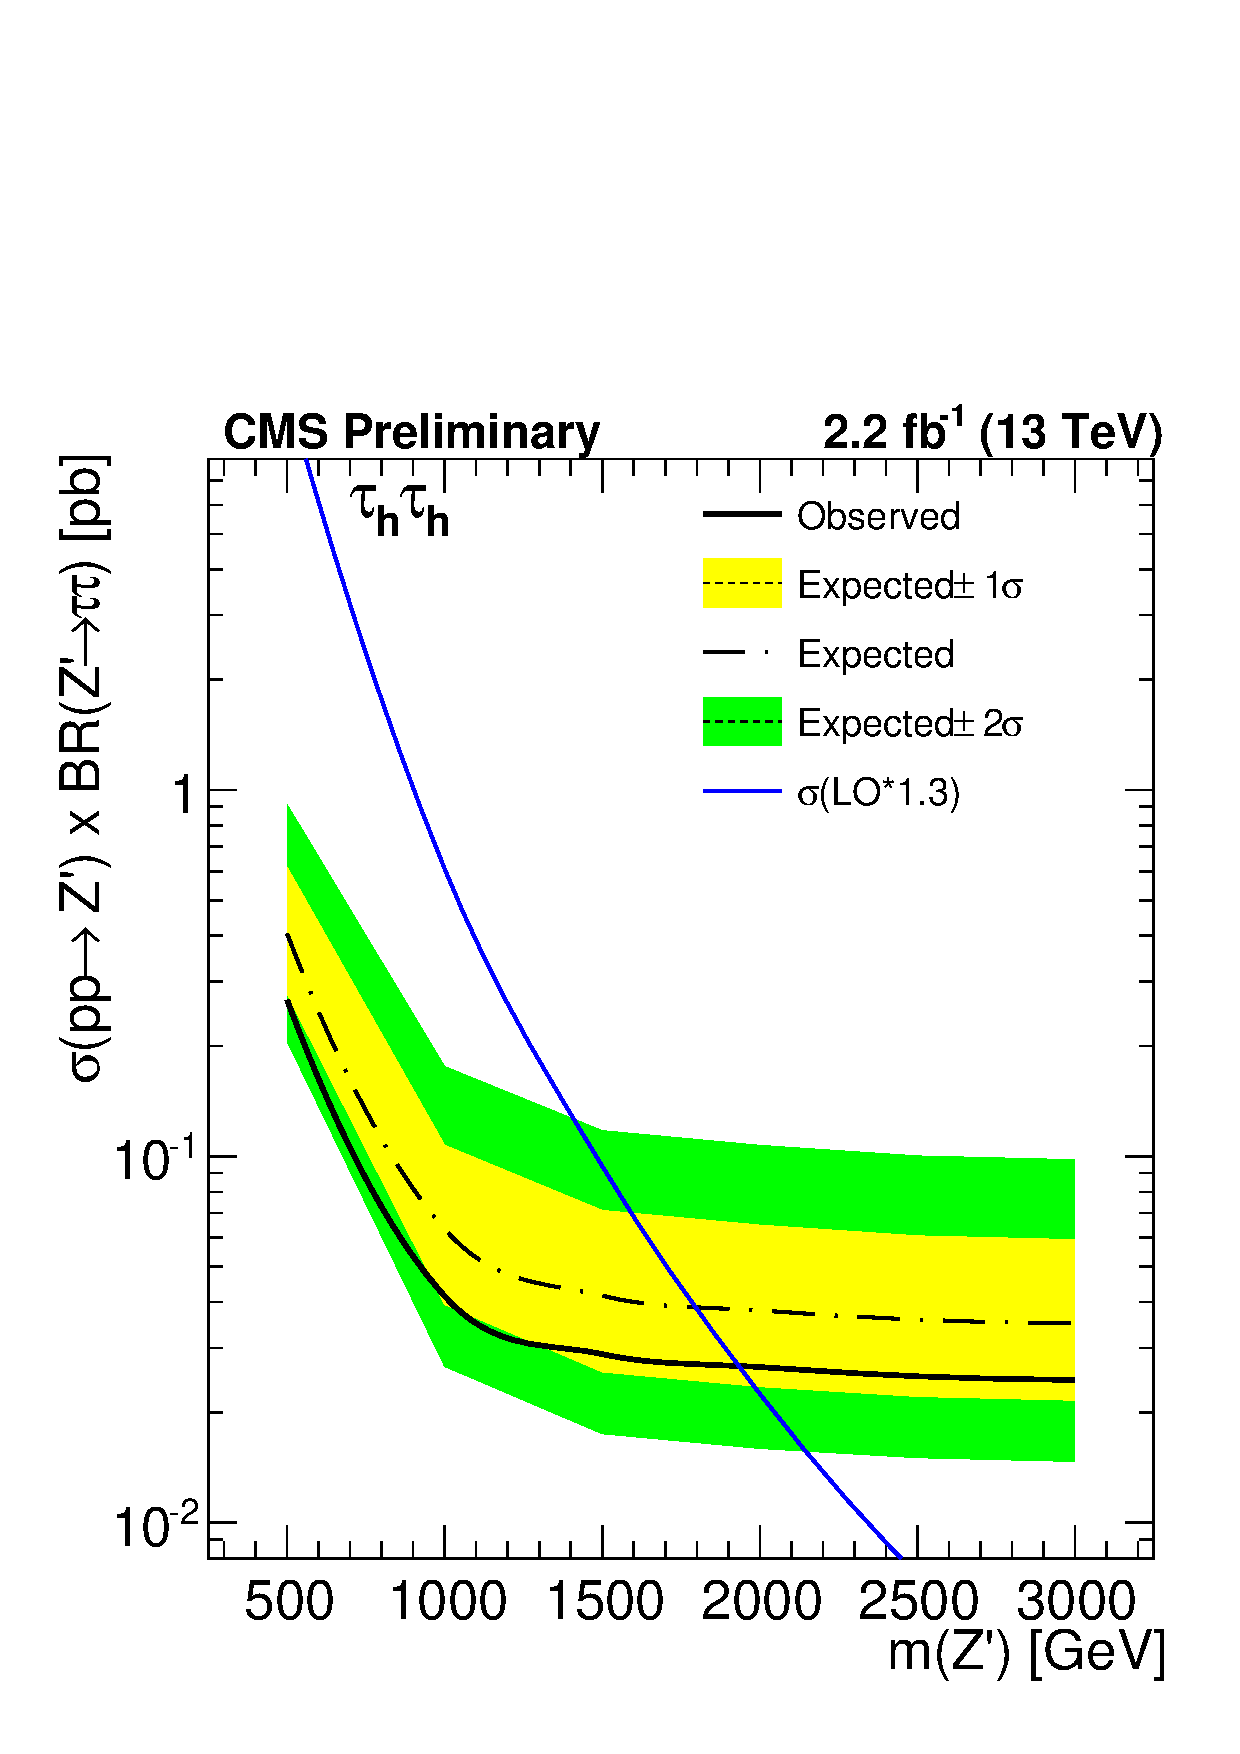
\includegraphics[width=0.5\textwidth]{figures/limits/Limit_TauTau}
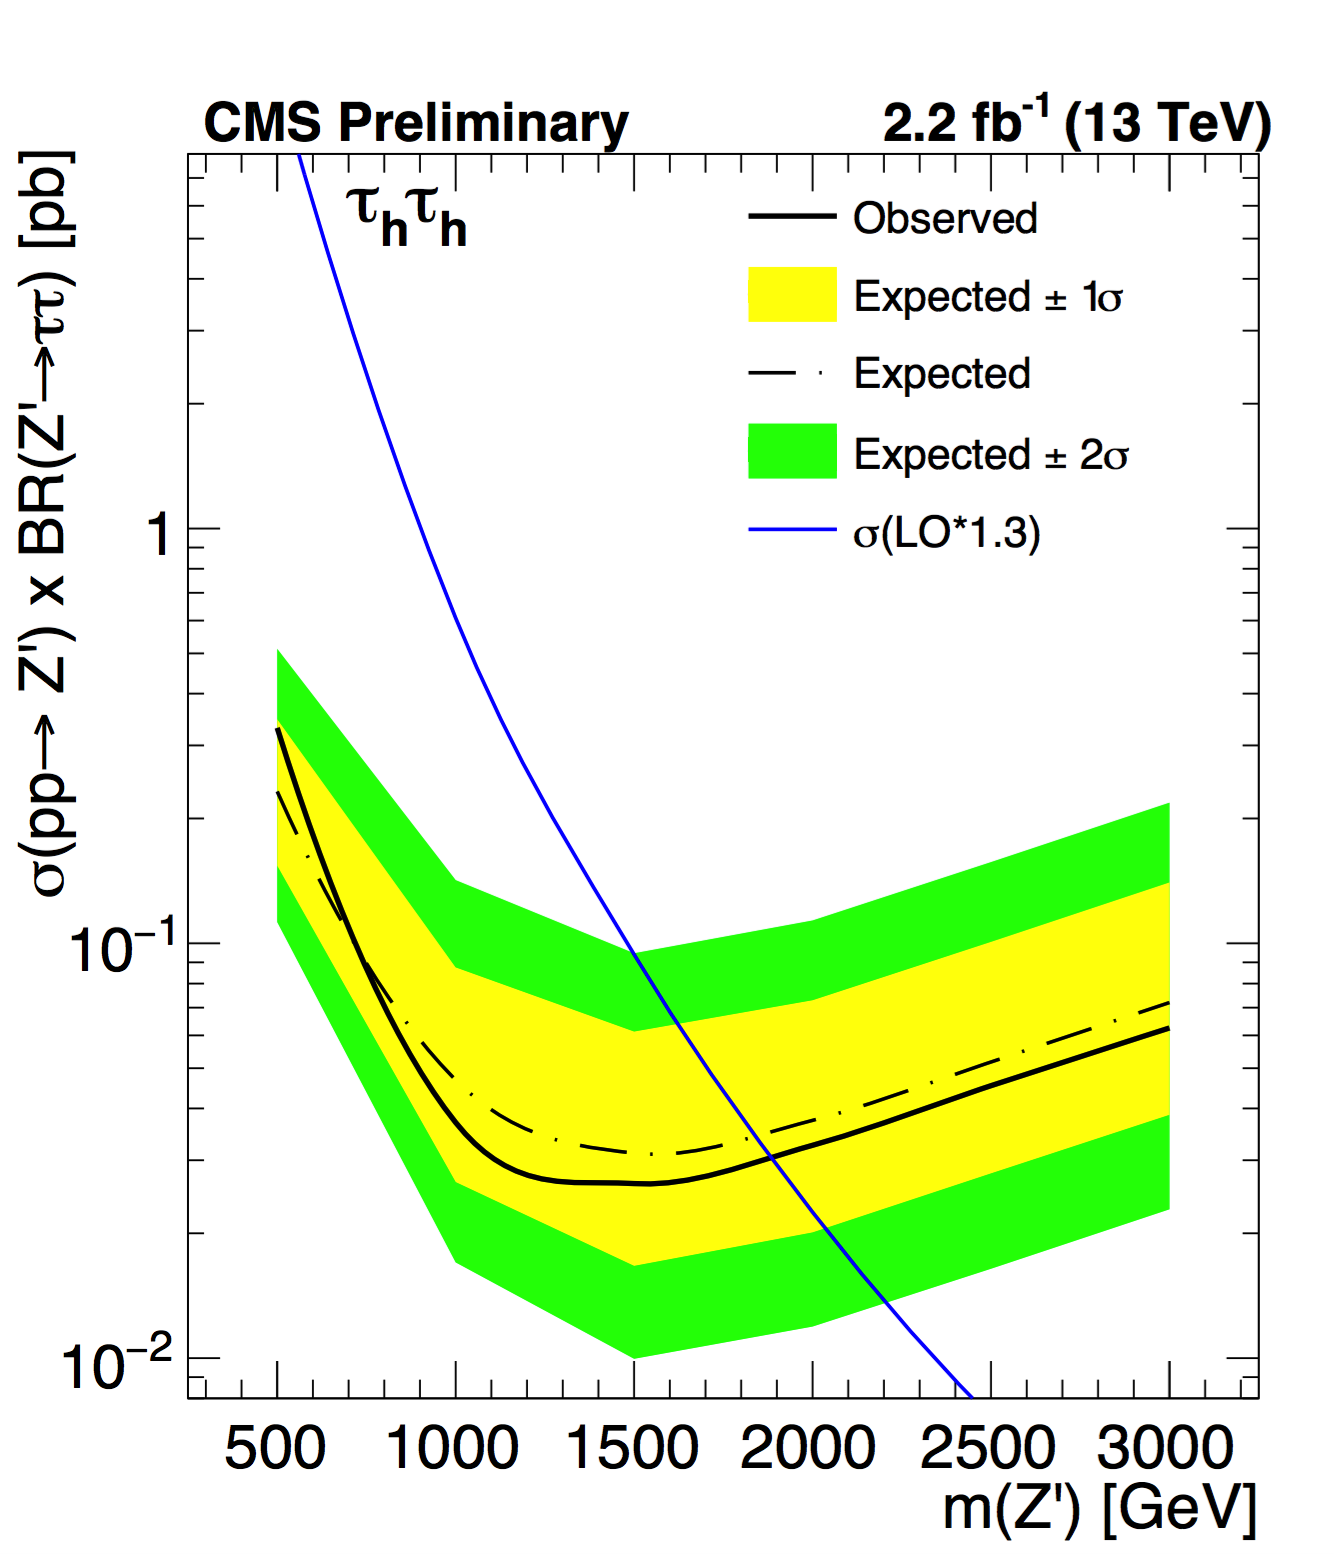
\includegraphics[width=0.5\textwidth]{figures/Limit_noLifetime.png}
%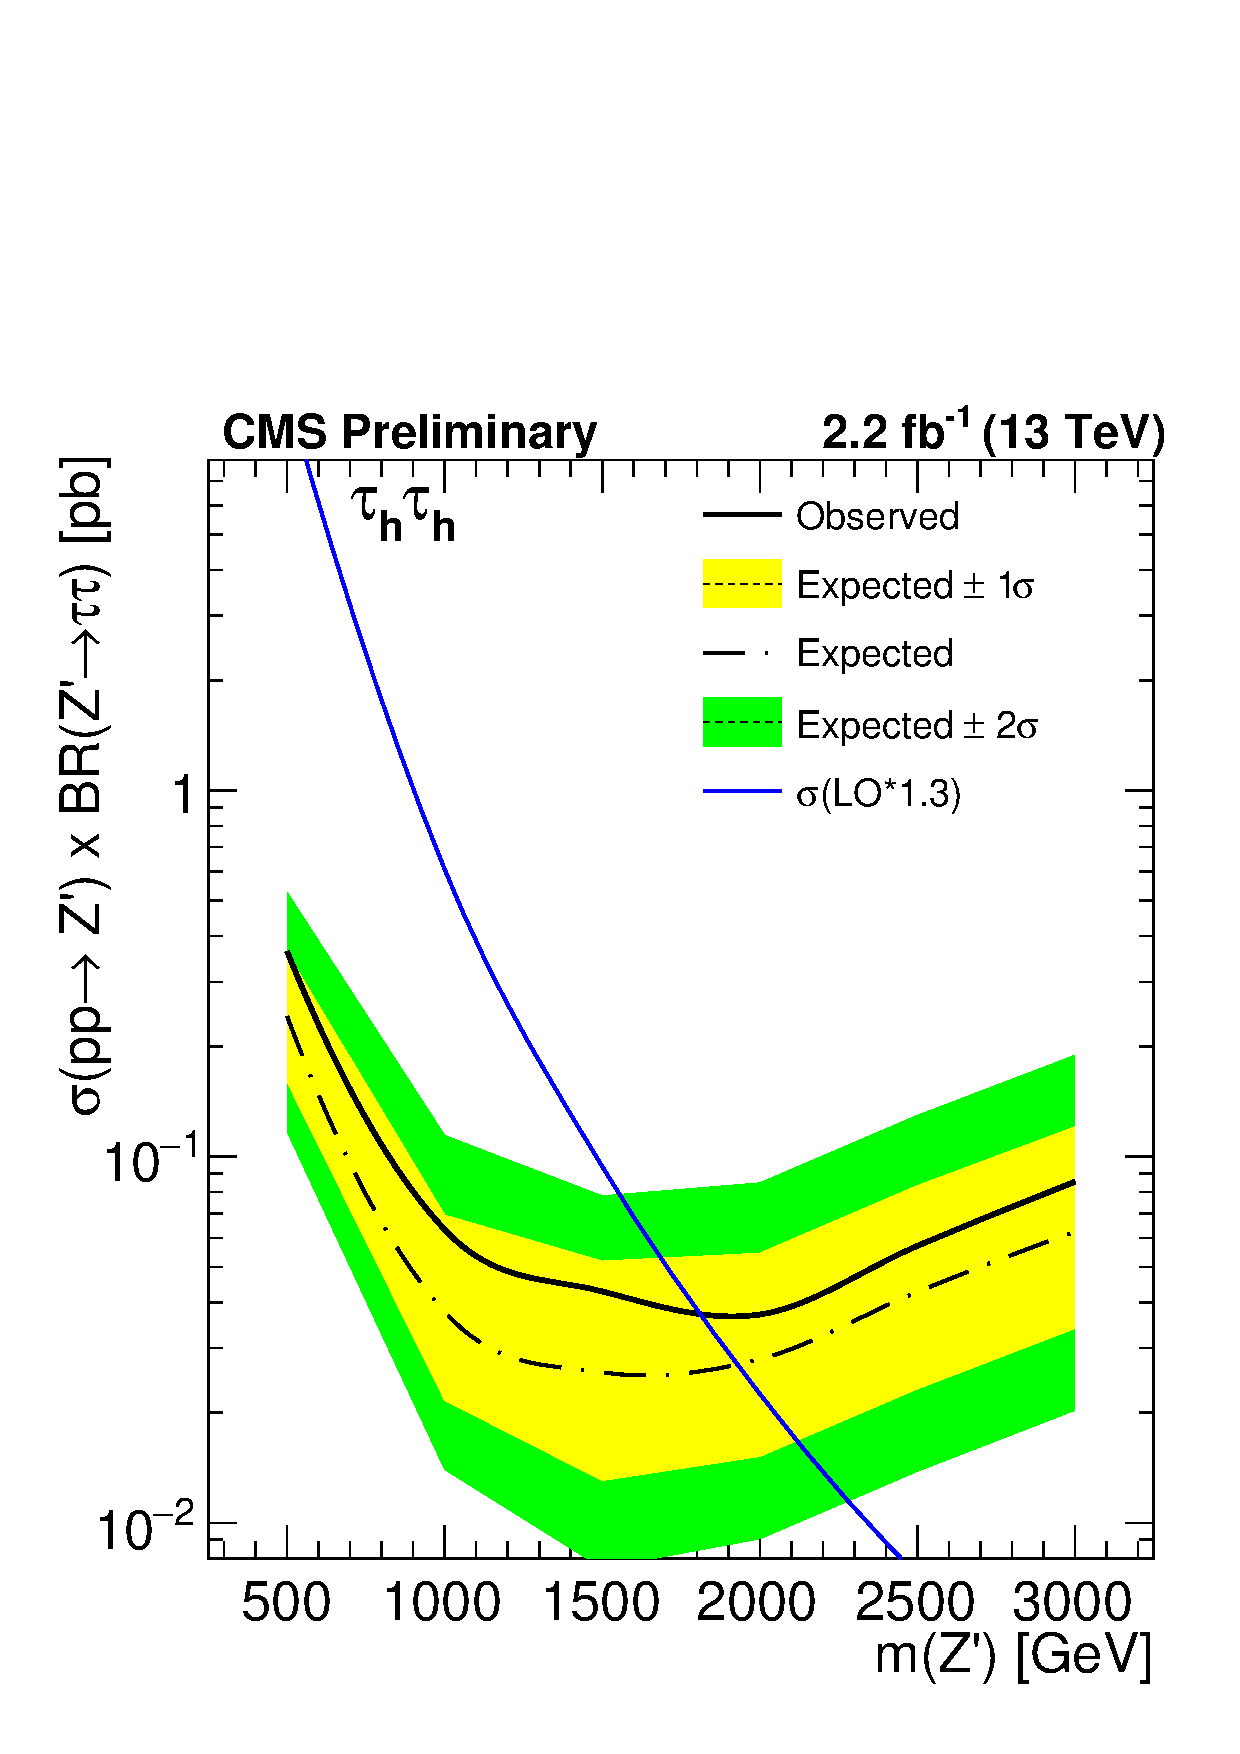
\includegraphics[width=0.5\textwidth]{figures/Limit_Lifetime_gt_2_NoPZeta_123prong.pdf}
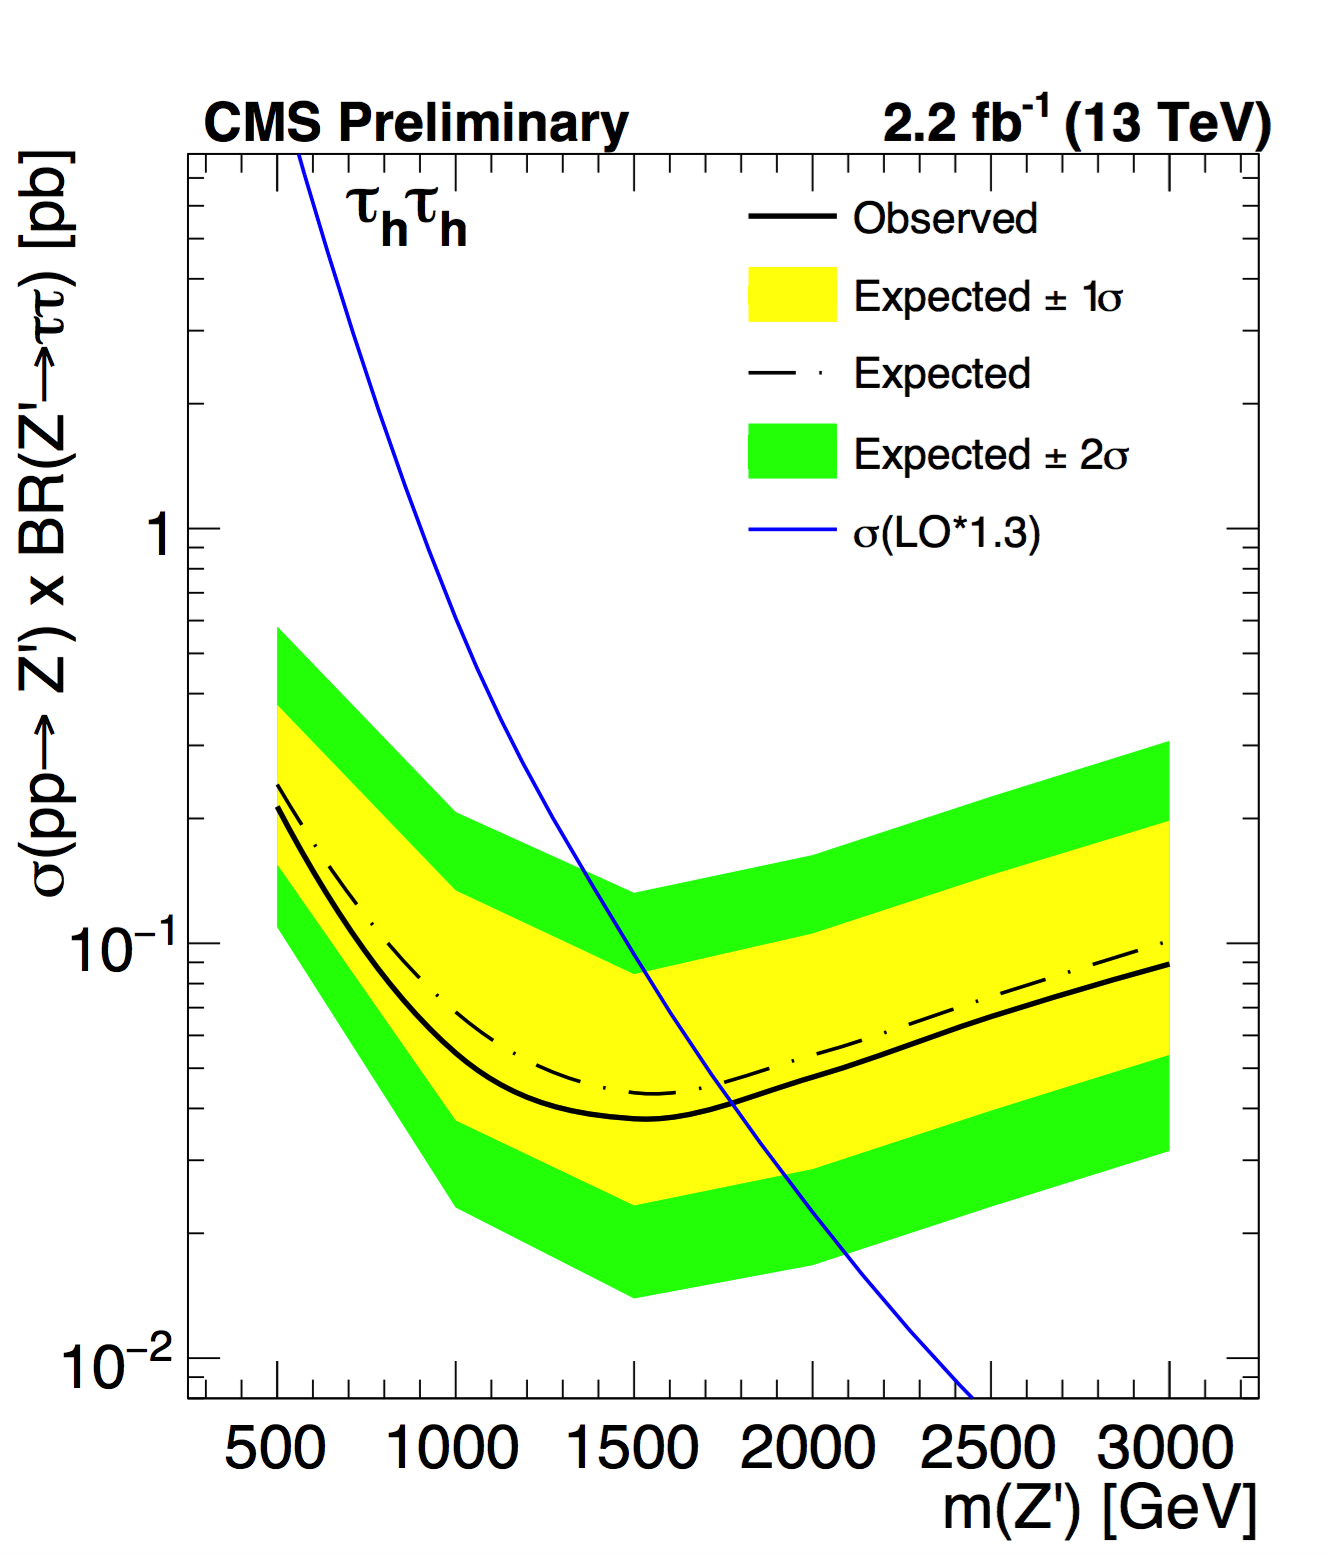
\includegraphics[width=0.5\textwidth]{figures/Limit_Lifetime_gt_3.png}
\caption{Limit calculated with standard 13 TeV selection sequence (top) compared with limit calculated with the standard selection sequence and a lifetime threshold of 3 applied (bottom).}
\label{fig:13TeVLifetimeLimits}
\end{figure}

\begin{figure}[tbh!]
\centering
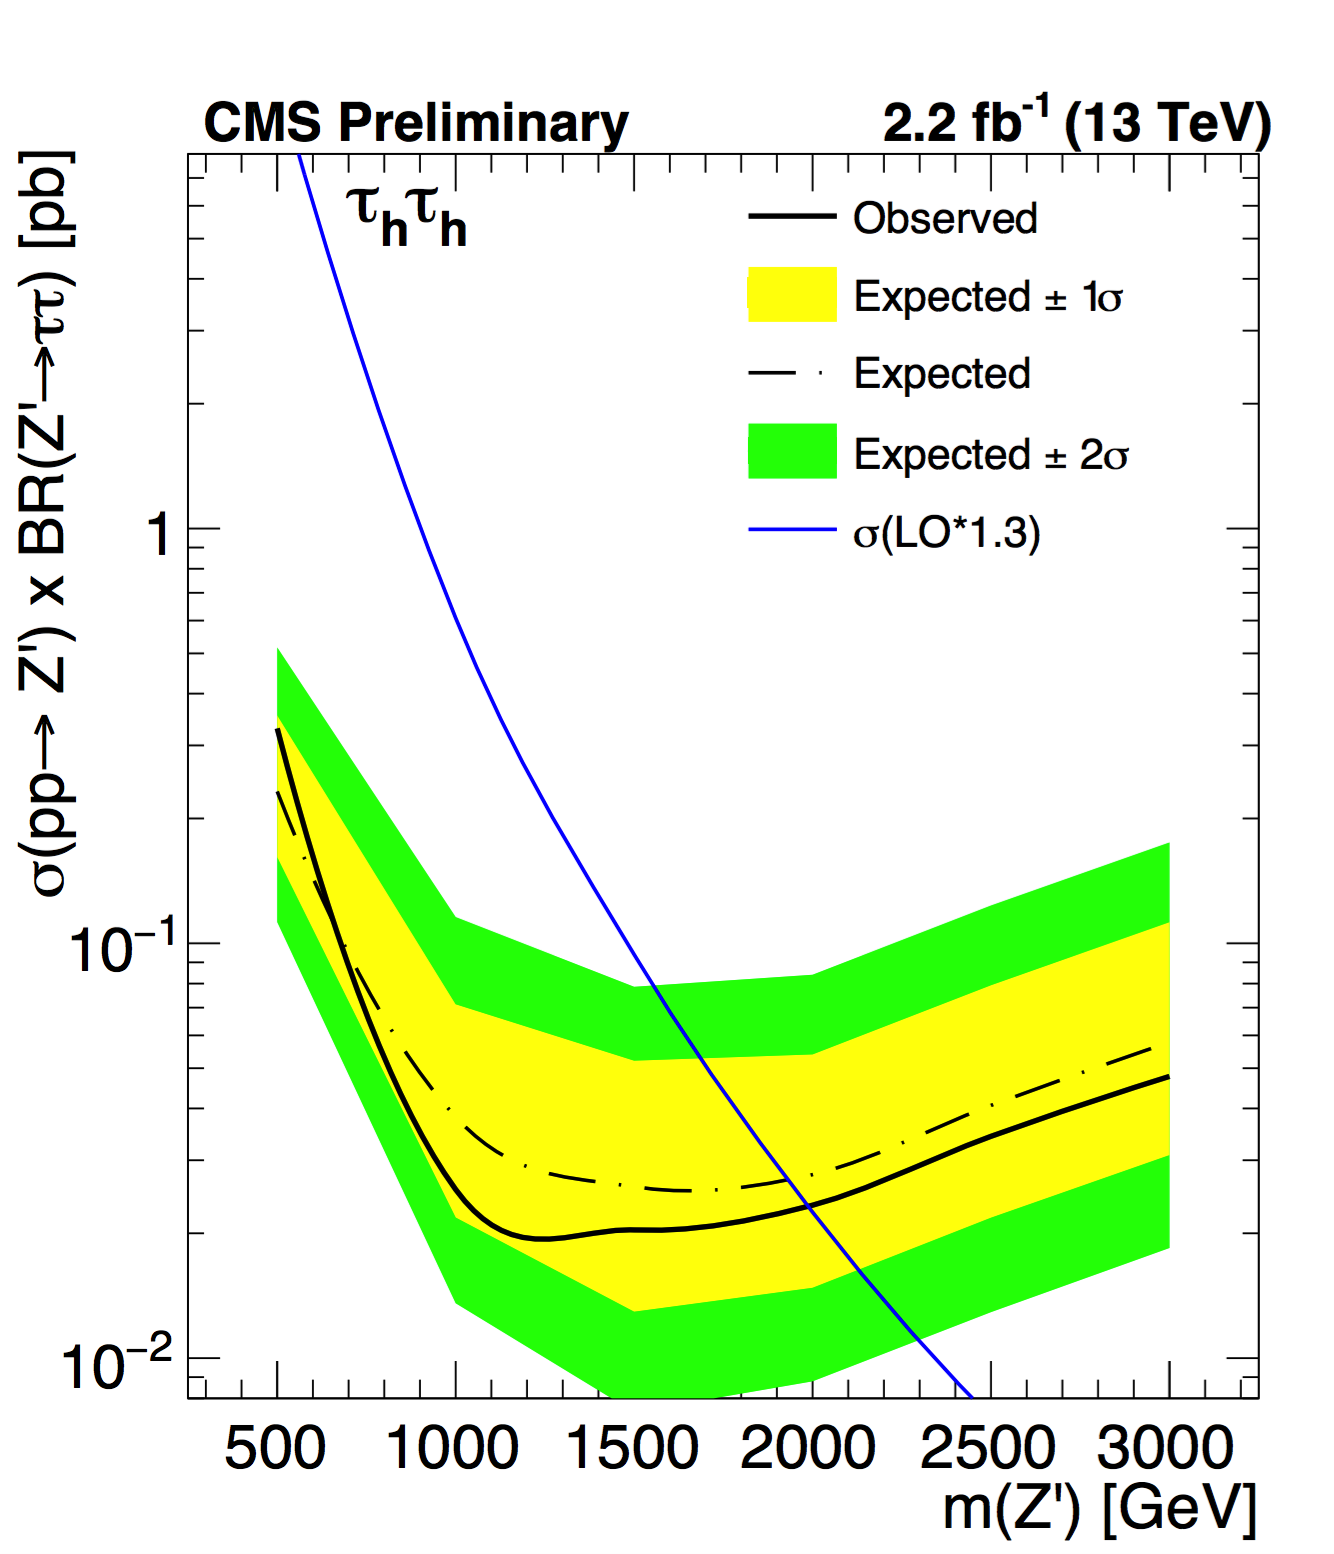
\includegraphics[width=0.5\textwidth]{figures/Limit_NoLifetime_NoPZeta_MET_gt_50.png}
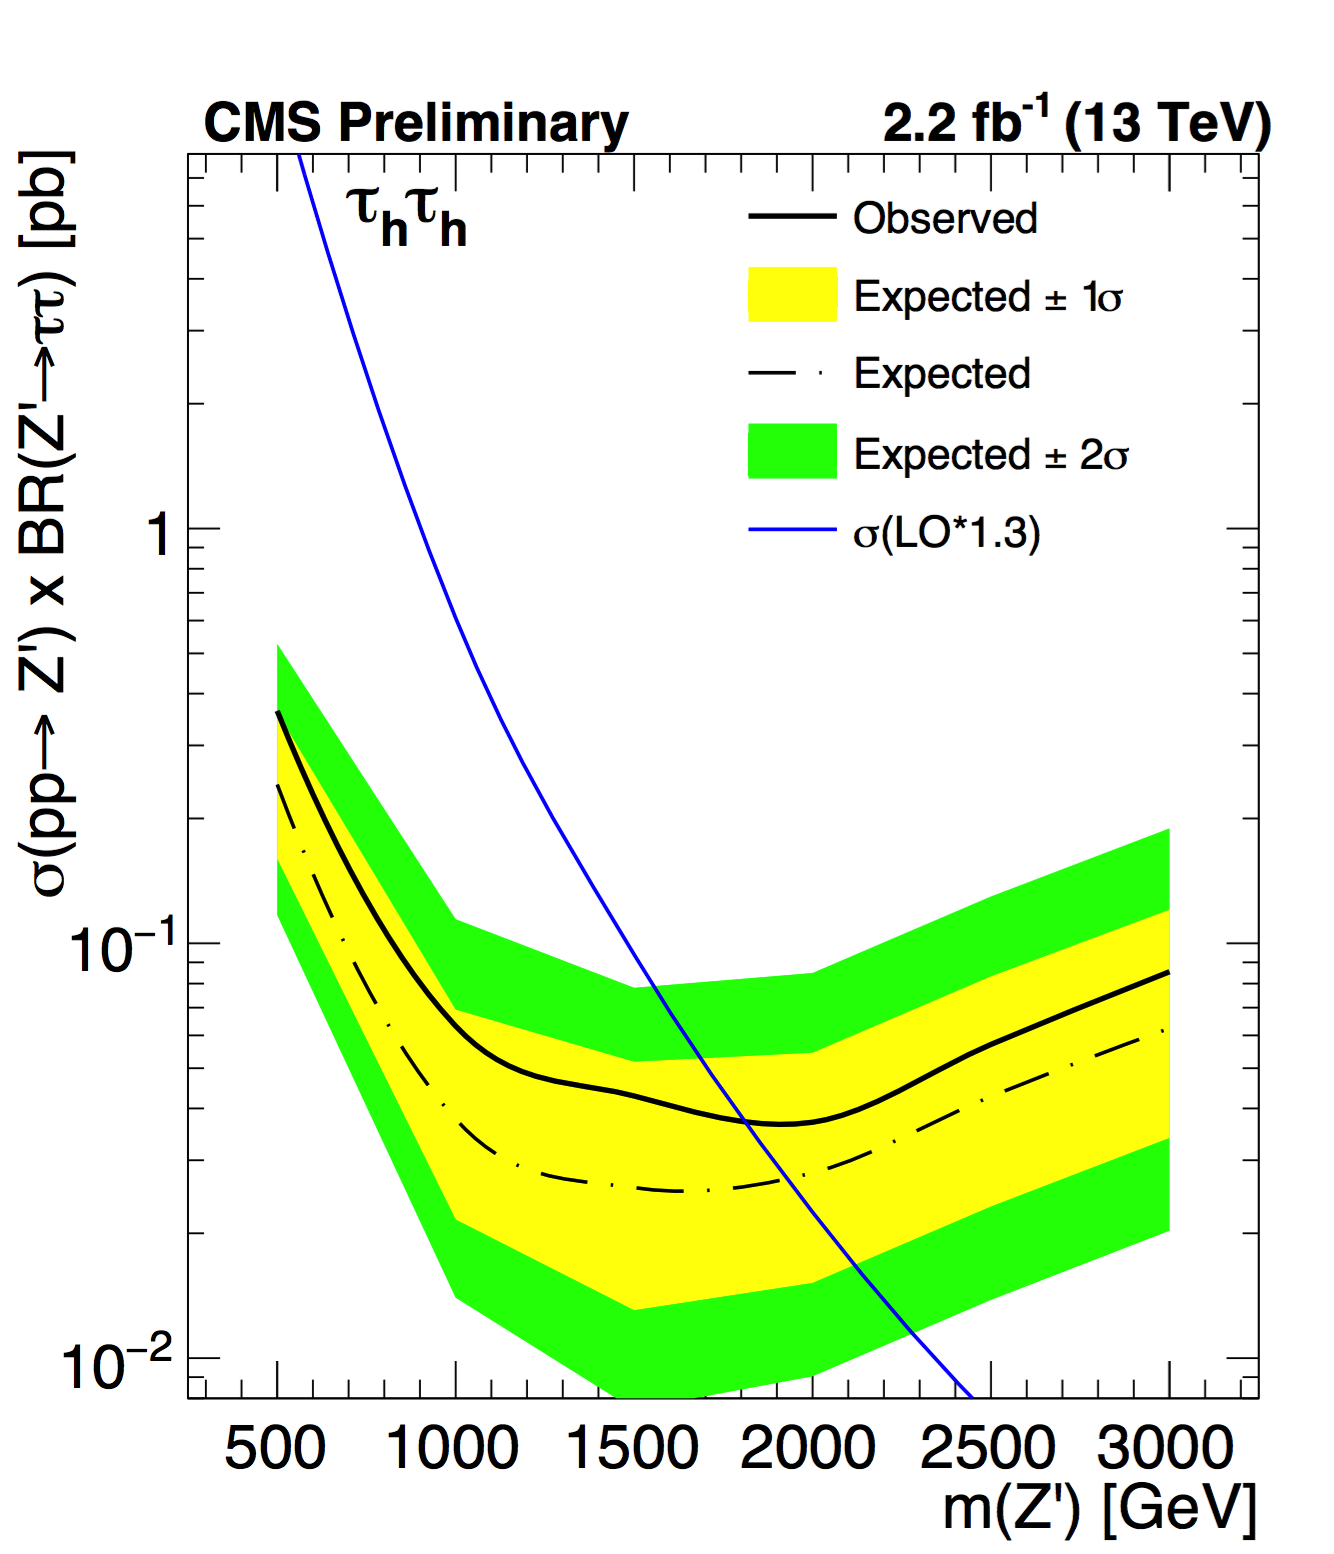
\includegraphics[width=0.5\textwidth]{figures/Limit_Lifetime_gt_2_NoPZeta_123prong.png}
\caption{Limit comparison with the $p_\zeta$ requirement removed and the $\MET$ minimum threshold increased to 50. The top plot has no lifetime threshold applied, while the bottom plot has a lifetime threshold of 2 applied. While the removal of $p_\zeta$ and the tightening of the $\MET$ threshold increases the baseline limit, the limit with the lifetime cut added is still lower (worse) than that without it applied.}
\label{fig:13TeVImprovedLimits}
\end{figure}
